% !TeX root = ../thesis.tex

\chapter{Einleitung}
\label{sec:introduction}

Die Kommunikation über das Medium Licht ist eine neue und äußerst vielversprechende Technologie aus dem Bereich der optischen, drahtlosen Kommunikation, die das sichtbare Spektrum für die Datenübertragung nutzt und sich aufgrund der hohen verfügbaren Bandbreite, des unregulierten sichtbaren Spektrums, und der nicht vorhandenen elektromagnetischen Interferenzen als Lösung für Funkkommunikationssysteme herauskristallisierte. Daneben wird das \gls{acr:OFDM} als Modulationsverfahren für \gls{acr:VLC} verwendet, da es in der Lage ist, hohe Datenraten zu erzielen und gleichermaßen mit einer hohen spektralen Effizienz zu übertragen. Zudem werden mithilfe jener die Auswirkungen von Störungen durch \gls{acr:ISI} reduziert.

\section{Motivation}
\label{sec:motivation}

Der wachsende Drang in der heutigen Zeit, mobil zu sein und die damit drastisch steigende Anzahl an Mobilfunkendgeräten, führt dazu, dass die elektromagnetischen Hochfrequenzbänder immer weiter überfüllt werden. Jedoch müssen Endgeräte jenes nutzen um mit anderen Geräten zu interagieren. In modernen, drahtlosen, mobilen Telekommunikationssystemen sind die gängigsten Technologien der Zugangsnetze zur Datenübertragung die Funkfrequenzen. Mit der steigenden Nachfrage an Hochgeschwindigkeitsdatendiensten steigt die Auslastung des \gls{acr:HF}-Spektrums. Darüber hinaus leidet die \gls{acr:HF}-basierte Kommunikation unter Mehrwegeausbreitung, was die Verfügbarkeit und Leistung von Verbindungen reduziert. Dies, zusammen mit der Überlastung des \gls{acr:HF}-Spektrums, bedeutet, dass nur wenige hochauflösende Kanäle in einem bestimmten Gebiet untergebracht werden können. Schätzungen zufolge finden etwa 70\% des drahtlosen Datenverkehrs in Innenräumen statt \cite{vlc2}. Daher müssen Alternativen für drahtlose Kommunikationssysteme, speziell in Innenräumen, in Betracht gezogen werden.
Eine solche Alternative sind \gls{acr:VLC}-Systeme, welche in ihren Anwendungsbereichen in Abbildung~\ref{fig:usecasevlc} illustriert werden. \gls{acr:VLC} nutzt das sichtbare Lichtspektrum, welches sich über eine Wellenlänge von 390 - 780nm erstreckt, und daher im Vergleich zur \gls{acr:HF}-Kommunikation eine etwa zehntausend mal höhere Bandbreite in der Terahertz Größenordnung bietet.\cite{ghassemlooyVisibleLightCommunications} 

\begin{figure}[H]
	\centering
	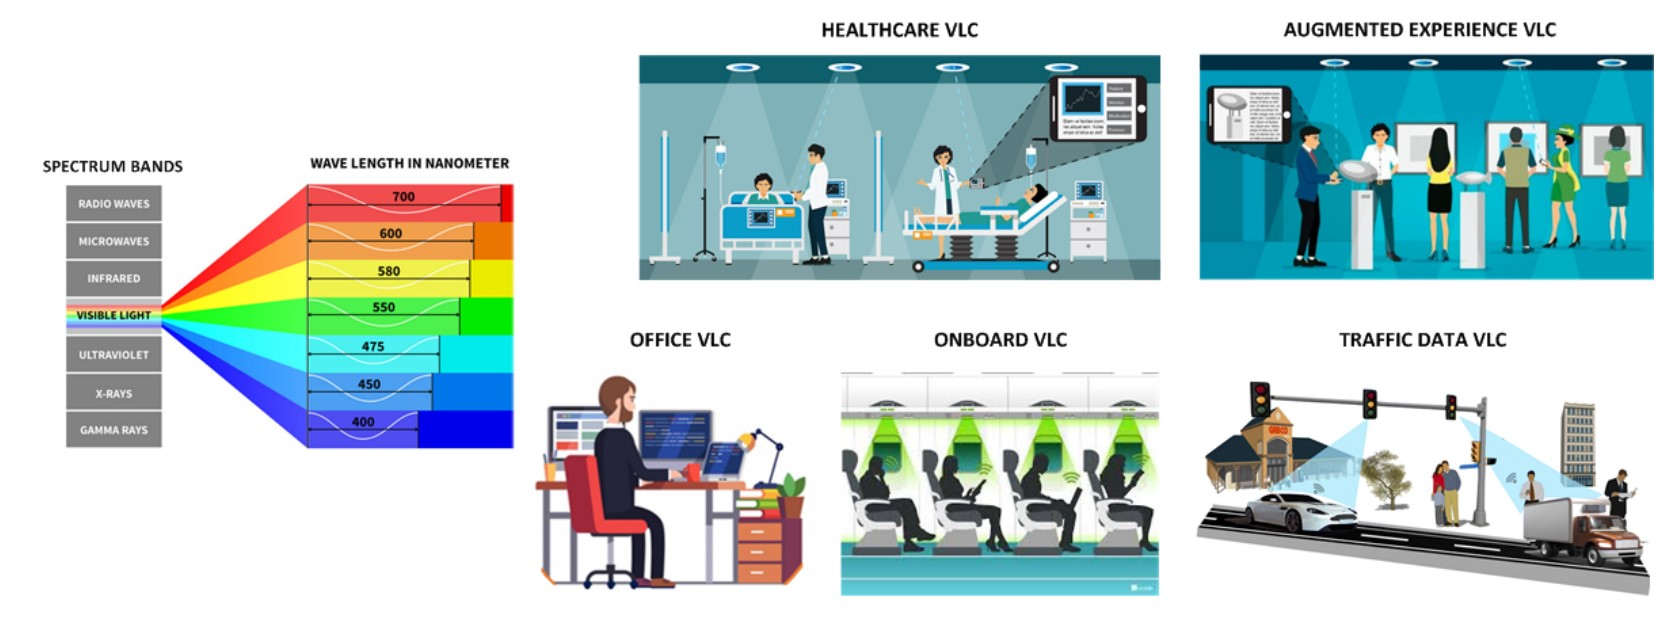
\includegraphics[width=1 \textwidth]{usecases.jpg}
	\caption[Wellenlänge und Use Cases von \gls{acr:VLC}]{Wellenlänge und Use Cases von \gls{acr:VLC}} 
	\cite{usecase}
	\label{fig:usecasevlc}
\end{figure}

Außerdem bietet es ein lizenzfreies Spektrum, nicht vorhandene elektromagnetische Interferenzen, und eine erhöhte Sicherheit für Innenraumsysteme, da Licht auf die Dimensionen seines Ausleuchtungskegels beschränkt ist. Darüber hinaus gilt \gls{acr:VLC} als ökologische Technologie, da \gls{acr:LED}s energieeffiziente und leicht steuerbare Lichtquellen sind.\cite{ghassemlooyVisibleLightCommunications} Außerdem werden die Vorteile von bereits implementierten \gls{acr:LED} für einen doppelten Zweck der Beleuchtung und der Datenkommunikation genutzt. Da moderne Kommunikationssysteme hohe Datenraten erfordern, muss ein Modulationsverfahren in Betracht gezogen werden, welches in der Lage ist, hohe Datenraten mit hoher spektraler Effizienz zu übertragen.\cite{vlc2} Hierbei wurde \gls{acr:OFDM} gewählt, welches im Laufe dieser Abschlussarbeit noch weiter eingeleitet und ausgeführt wird.


\section{Ziel der Arbeit}
\label{sec:The aim of the work}


Ziel dieser Abschlussarbeit ist es, einen \gls{acr:VLC}-Sender mit einem variablen Offset für den Lichtstrom und einer automatischen Amplitudenregelung aufzubauen. Dieser soll es ermöglichen, mittels modulierter Lichtwellen, Audio Daten von \gls{acr:PC} zu \gls{acr:PC} zu übertragen. Dazu wurden folgende Rahmenbedingungen festgelegt: 

\begin{itemize}
	\item Simulation der analogen Signalverarbeitungsschaltung in LT-Spice
	\item Projektierung einer Platine für die Komprimierung der Schaltungsgröße
	\item Konstruktion eines Gehäuses für die Unterbringung der Hardwarekomponenten
	\item Auseinandersetzung mit dem thermischen Management
	\item Variabilität des Offsets zur Steuerung des Lichtstroms
	\item Programmierung einer automatischen Amplitudenregelung
	\item Modulation und Demodulation des Audio-Sendesignals mittels Dream Software
\end{itemize}




\section{Vorgehensweise}
\label{sec:method}
Zunächst wurde eine allgemeine Literaturrecherche zum Thema \gls{acr:VLC} angestellt, welche dazu dienen sollte sich einen Überblick über die gegebene Thematik zu verschaffen. Im Anschluss konnte durch das dadurch erlangte Wissen, die Simulation einer notwendigen analogen Signalverarbeitungsschaltung simuliert und dementsprechend theoretisch erprobt werden. Nach Beendigung der Simulation wurde die Schaltung zur Durchführung einer Funktionsprüfung auf einem sogenannten Breadboard aufgebaut. Nach dem sich dieser Prototyp sowohl in der analogen Signalübertragung, als auch im Zusammenspiel mit der digitalen Signalverarbeitungssoftware und Programmierung als funktionell bewährte, konnte ein Platinenlayout erstellt werden. Anschließend wurde die Planung eines Gehäuses durchgeführt, bei welcher viele Faktoren als Rahmenbedingungen vorgesehen wurden. Zu diesen galten unter anderem ein platzsparendes Design und eine gute Wärmeabführung der Leistungsbauteile. Zuletzt konnten Übertragungsstrecken aufgebaut und anhand von Kriterien wie dem maximalen Datendurchsatz und verschiedener Übertragungsentfernungen evaluiert wurden. 

